\documentclass{beamer} %[12pt,handout]

\usepackage[english]{babel}
\selectlanguage{english}
\usepackage[utf8]{inputenc}
\usepackage{hyperref}
\usepackage{url}
\usepackage{csvsimple}
\usepackage{bera}% optional: just to have a nice mono-spaced font
\usepackage{listings}
\usepackage{xcolor}
\usepackage{graphicx}

\colorlet{punct}{red!60!black}
\definecolor{background}{HTML}{EEEEEE}
\definecolor{delim}{RGB}{20,105,176}
\colorlet{numb}{magenta!60!black}

\lstdefinelanguage{json}{
    basicstyle=\normalfont\ttfamily,
    numbers=left,
    numberstyle=\scriptsize,
    stepnumber=1,
    numbersep=8pt,
    showstringspaces=false,
    breaklines=true,
    frame=lines,
    backgroundcolor=\color{background},
    literate=
     *{0}{{{\color{numb}0}}}{1}
      {1}{{{\color{numb}1}}}{1}
      {2}{{{\color{numb}2}}}{1}
      {3}{{{\color{numb}3}}}{1}
      {4}{{{\color{numb}4}}}{1}
      {5}{{{\color{numb}5}}}{1}
      {6}{{{\color{numb}6}}}{1}
      {7}{{{\color{numb}7}}}{1}
      {8}{{{\color{numb}8}}}{1}
      {9}{{{\color{numb}9}}}{1}
      {:}{{{\color{punct}{:}}}}{1}
      {,}{{{\color{punct}{,}}}}{1}
      {\{}{{{\color{delim}{\{}}}}{1}
      {\}}{{{\color{delim}{\}}}}}{1}
      {[}{{{\color{delim}{[}}}}{1}
      {]}{{{\color{delim}{]}}}}{1},
}

  \hypersetup{
    pdfauthor={Georges Alkhouri, Tom Neumann},
    pdftitle={Final Presentation - Dockerizing Linked Data}
  }

\usetheme{default}
\setbeamercolor{title}{fg=black}
\setbeamercolor{frametitle}{fg=black}
\setbeamercolor{description item}{fg=black}
\setbeamercolor{itemize item}{fg=black}
\setbeamercolor{bibliography entry author}{fg=black}
\setbeamercolor{bibliography entry title}{fg=black}
\setbeamercolor{bibliography entry location}{fg=black}
\setbeamercolor{bibliography item}{fg=black}
\setbeamercolor{caption name}{fg=black}

\setbeamertemplate{itemize items}[circle]
%\setbeamertemplate{caption}{
%\begin{beamercolorbox}[wd=.5\paperwidth, sep=.2ex]{block body}\insertcaption
%\end{beamercolorbox}
%}

\addtobeamertemplate{frametitle}{\vskip+5.0ex}

\beamertemplatenavigationsymbolsempty

\setbeamertemplate{footline}[frame number]

\begin{document}

\title{Final Presentation - Dockerizing Linked Data}
\author{Georges Alkhouri, Tom Neumann}
\institute{University of Applied Sciences Leipzig}
\date{6th Jul. 2015}

\frame{\titlepage}

\frame{

\frametitle{Problem}

Populare knowledge bases faceing \textbf{performence/availability} issues through \textbf{high request} rates
\vspace{\baselineskip}

\centerline{Solution $\downarrow$} 

\vspace{\baselineskip}
Run a local mirror of the knowledge base with a SPARQL endpoint
}

\frame{

\frametitle{New Problem}

To run and maintain a local knowledge base environment is a complex task requiring a lot of effort and is not suitable for domain admins who just want to use the SPARQL interface
\vspace{\baselineskip}

\centerline{New Solution $\downarrow$} 

\vspace{\baselineskip}

\centerline{\textbf{Dockerizing Linked Data}}
}

\frame {
\frametitle{Usage Example: Professorenkatalog}

The Catalogus Professorum Lipsiensium

\begin{itemize}

\item Knowledge base of professors at the Leipzig University
\item Includes records from 1409 to presence
\item Comprises over 14, 000 entities
\item Many interlinked connections in the LOD Cloud
\item Curated by \textbf{historical researchers} and \textbf{interested citizen scientists}

\end{itemize}
}

\frame {
\frametitle{Usage Example: Professorenkatalog}
\framesubtitle{Infrastructure}

Professorenkatalogs infrastructure consists of several web applications (Presentation, Storage, Backup, ... )

}

\frame{

\begin{figure}
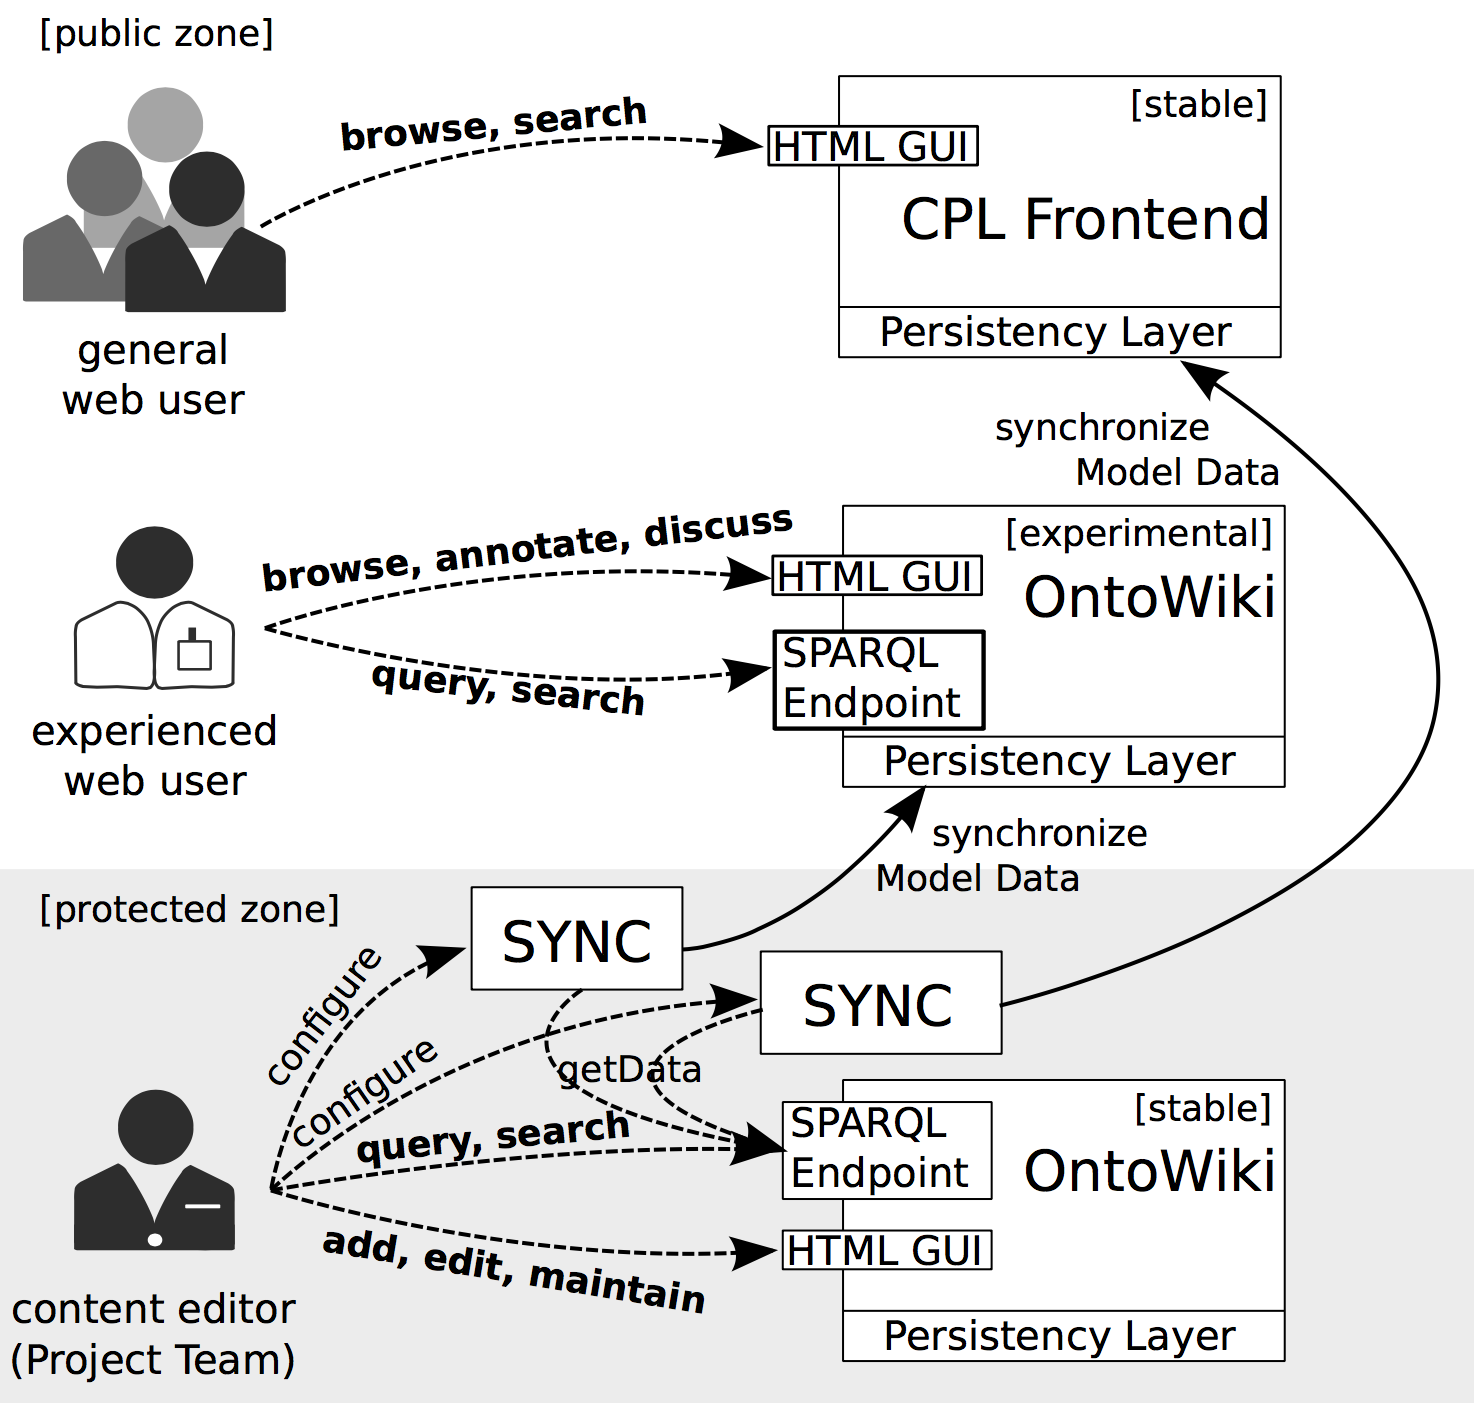
\includegraphics[scale=0.32]{CPL.png}
\caption{Architecture of Professorenkatalog\cite[p. 6]{dld-paper}}
\end{figure}

}

\frame {
\frametitle{References}

\begin{thebibliography}{Knowledge Base Shipping to the Linked Open Data Cloud}
	\setbeamertemplate{bibliography item}[text]
      		\bibitem[1]{dld-paper}
        	Knowledge Base Shipping to the Linked Open Data Cloud
 		\newblock {\em Natanael Arndt, Markus Ackermann, Martin Brümmer, Thomas Riechert}
		\newblock{Jul. 2015}
\end{thebibliography}

}

\end{document}